\section{模型的横向对比与择优}

前面各问都在同一套分布参数框架内求解，但这一框架本身是否必要，需要与更简单的做法比过之后才能回答。本章构造两个简化候选并与本文模型放在同一条件下实算：同一求解器、同一网格、同一时间步安排、同一组题给数据。唯一无法完全统一的是判据，因为最简的候选没有径向坐标，逐点判据在它那里无法定义——这一点本身就是对比的结论之一。

\subsection{候选模型的构造}

第一个候选是集中参数模型，即把整根药材视为一个没有内部梯度的点，只追踪截面平均含水率的演化。这类薄层模型在干燥文献中用于拟合失水曲线，其前提是内部阻力可略\upcite{boeri2012thinlayer}。对圆柱作整体水量平衡可得

\begin{equation}
\frac{\mathrm{d}\bar C}{\mathrm{d}t}=-\frac{2h_m}{R_0}\big[\bar C(t)-C_a(t)\big],
\qquad
\tau=\frac{R_0}{2h_m}=12500\ \mathrm{s}=3.4722\ \mathrm{h},
\label{eq:lumped}
\end{equation}

时间常数 $\tau$ 完全由表面传质决定。式~\eqref{eq:lumped} 用同样的后向 Euler 推进，判据退化为 $\bar C<0.15$，得停时 $11.1669$~h；若进一步把空气水分浓度固定为平台值，可写出闭式解并得 $11.1763$~h，两者相差 $0.08\%$，说明该分支的数值实现无误，$11.1669$~h 确实是这个模型的答案而不是算错的结果。

第二个候选保留一维径向分布，只把物性冻结为常数。冻结状态必须在求解之前选定，本文取题面直接给出的初始态 $C=2.55$~kg/kg、$T=28$~°C，对应 $D=5.642\times10^{-9}$~m$^2$/s；这一选取本身带有任意性，其后果在本节末一并讨论。其余设置与问题三完全相同，得停时 $22.5636$~h，穿越区间为 $81180$ 至 $81240$~s（判据量 $0.150215\to0.149952$），终态截面平均含水率 $0.1158$~kg/kg、表面 $0.0861$~kg/kg。该分支在 $N=40$ 与 $N=80$ 上一致到 $10^{-3}$~h，因此它与本文结果的差距不是网格造成的。四个模型的指标汇总于表~\ref{tab:compare}。

\begin{table}[H]
\centering
\caption{四个候选模型在同一条件下的实算对比}\label{tab:compare}
% 六列宽表：列间距由默认 6pt 收到 4pt，十二个列间共省 24pt，足以消掉横向溢出。
\setlength{\tabcolsep}{4pt}
\begin{tabular}{llcccc}
\toprule
模型 & 结构 & $t_{\rm dry}$/h & 折合/d & 落在 2--3~d 内 & $C(0)-C(R)$ \\
\midrule
M1 集中参数     & 零维常微分方程 & 11.1669 & 0.47 & 否 & 恒为 $0$ \\
M2 常物性一维   & 一维径向       & 22.5636 & 0.94 & 否 & 0.0639 \\
M3 变物性一维   & 一维径向       & 57.5316 & 2.40 & 是 & 0.0974 \\
M4 变物性加动边界 & 一维加动边界 & 51.1384 & 2.13 & 是 & 0.0974 \\
\bottomrule
\end{tabular}
\end{table}

四个停时相差极大，最长的 M3 与最短的 M1 之间差 $5.15$ 倍，说明模型选择不是精度上的微调而是量级上的取舍。图~\ref{fig:model-compare} 把四条平均含水率轨迹与各自的停时画在一起。

\begin{figure}[htbp]
  \centering
  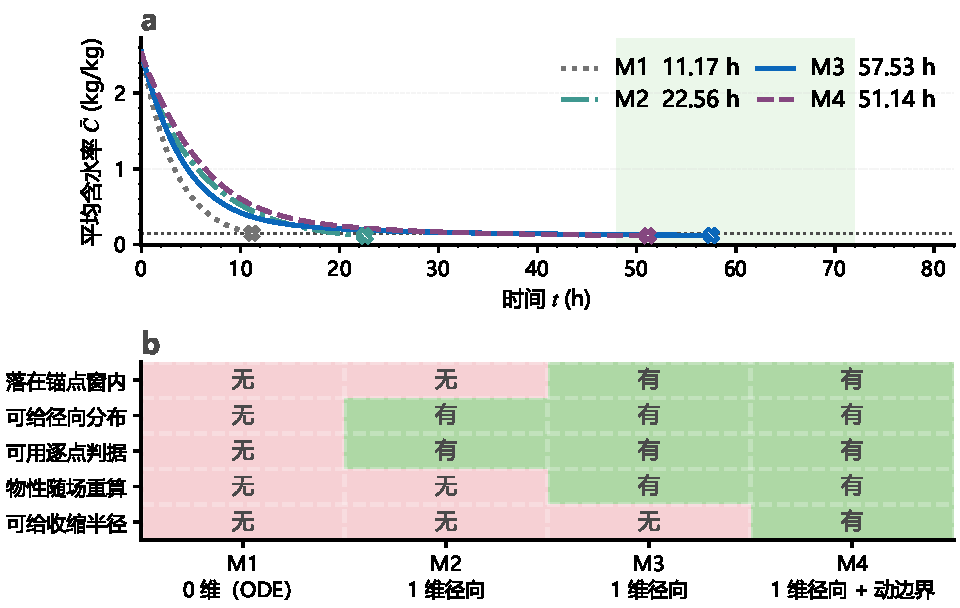
\includegraphics[width=0.9\textwidth,height=0.8\textheight,keepaspectratio]{../figures/fig_model_compare.pdf}
  \caption{四个候选模型的横向对比。a：M1—M4 的平均含水率轨迹与各自判据下的
  停时（圆点），灰带为题面所给 2—3 d 外部参考窗口换算的时间区间，只有 M3、
  M4 的停时落在窗内。b：能力矩阵，逐格标记该模型是否具备对应能力；其中“落在
  参考窗内”一行即指 a 图灰带。逐级叠加常物性、变物性、变物性加收缩三档，可
  分离出各档对停时的贡献，并说明为何取 M4 为主模型。}
  \label{fig:model-compare}
\end{figure}

左图中四条轨迹在最初一两个小时几乎重合，此后迅速分开：M1 一路保持指数衰减的形状，M2 的下降在中段就开始变缓，M3 与 M4 则拖出一条长尾。分离发生的时刻正是含水率降到 $1$~kg/kg 附近、扩散系数开始明显下滑的时刻，这说明四者的差距并非来自初始设置而是来自对干燥后期的刻画。两条简化轨迹的停时圆点都落在灰带左侧很远处，M3 与 M4 的圆点落在带内。右图逐格给出四个模型在径向分辨、逐点交付、参考窗、守恒精度四项上的表现，可以看出被排除的两个候选各自缺失的不是同一项。

\subsection{排除简化模型的定量依据}

集中参数模型被排除有三条各自独立的理由。其一是适用性判据：传质毕奥数 $\mathrm{Bi}_m=h_mR/D$ 的全过程实测区间为 $1.490$ 至 $5144$；即便把分母换成四个参考状态中最大的扩散系数，取到比实测下界更宽松的 $1.188$，也已是集中参数适用上限 $0.1$ 的 $11.9$ 倍，内部扩散阻力在任何时刻都不可忽略。其二是结构性缺陷：式~\eqref{eq:lumped} 中根本不出现扩散系数，因此它无法表达本题的核心机制——变干使扩散系数崩塌、外层结壳把水分锁在内部。其三是交付能力：题目要求给出每 $0.1$~cm 的逐点水分场，而该模型只有一个平均值，连输出形式都无法满足。实算 $11.1669$~h 只有本文结果的 $19.4\%$，把远未干透的药材判为合格。

常物性模型被排除的理由不同，它有径向分布，缺陷在于答案取决于建模者的选择而非题给数据。扩散系数在四个同样说得通的参考状态之间相差 $4330$ 倍：初始态 $(2.55,28\,^\circ\mathrm{C})$ 为 $5.642\times10^{-9}$，高温初期 $(2.55,50\,^\circ\mathrm{C})$ 为 $1.347\times10^{-8}$，判据阈值处 $(0.15,50\,^\circ\mathrm{C})$ 为 $8.001\times10^{-10}$，达标时的表面态 $(0.0526,50\,^\circ\mathrm{C})$ 为 $3.111\times10^{-12}$；实算全程的扩散系数跨越 $3.60$ 个数量级。冻结在其中任何一个状态都同样有理由，而不同的选择会使停时大幅摆动，这样的模型无法自证。冻结在初始态相当于把末期的扩散能力系统性高估三个数量级，因而给出偏早的 $22.5636$~h。

\subsection{变物性的净贡献与两个主模型的关系}

把 M2 与 M3 对照可以直接读出变物性这一项的价值：其余设置全部相同，仅让四个系数按附录 3 随解变化，停时便由 $22.5636$~h 变为 $57.5316$~h，相差 $2.55$ 倍。这个倍数说明变物性不是为复杂而复杂，它改变的是结论的量级；同时也说明表~\ref{tab:compare} 中 M2 的径向落差 $0.0639$ 小于 M3 的 $0.0974$~kg/kg——冻结高估的扩散能力不仅缩短了时间，还把内外差别一并抹平了。

M3 与 M4 之间不存在择优问题。题目对问题三与问题四分别指定了物性附录与是否收缩，两者是对两个不同设问的回答，各自都通过了同一组适用性判据与守恒检验。它们的差别已在第~\ref{sec:q34} 小节按物性与几何两项分解，此处不再重复。就本文的主线而言，能同时满足适用性判据、落在题面给出的参考区间、并给出题目所要求的逐点场这三项的，只有 M3 与 M4；两个简化候选各自在其中至少两项上失败。
